% !TeX encoding = UTF-8
% !TeX program = pdflatex

\documentclass[11pt]{article}
\usepackage{graphicx}

\title{{\bf Understanding the Galois/Counter Mode (GCM)} \\ \bigskip \large HW3 - CNS Sapienza}
\date{2019-11-21}
\author{Valerio Coretti 1635747}
\pagenumbering{roman}

\begin{document}
\maketitle

\section{Introduction}
Many developers make the mistake of only encrypting data without any considerations about the integrity. But this makes the road easier for an attacker. For this reason in this paper we want talk about {\em Authenticated Encryption (AE)}.

AE is an encryption system which provides both data confidentiality and data integrity assurances to the information being protected. In addition to protecting message, it can provide security against {\em chosen ciphertext attack}. In these attacks, an adversary attempts to gain an advantage against a cryptosystem (e.g., information about the secret decryption key) by submitting carefully chosen ciphertexts to some "decryption oracle" and analyzing the decrypted results. Authenticated encryption schemes can recognize improperly-constructed ciphertexts and refuse to decrypt them.

Now we need to talk about {\em Authenticated encryption with associated data (AEAD)}.
AEAD is a variant of AE that allows a recipient to check the integrity of both the encrypted and unencrypted information in a message. AEAD binds associated data (AD) to the ciphertext. It is required, for example, by network packets. The header needs integrity, but must be visible; payload, instead, needs integrity and also confidentiality. Both need authenticity.

In the following sections we will talk about a mode of operation called Galois/Counter Mode (GCM) that is an algorithm designed to provide both data integrity and confidentiality. In particular we will analyze the main mechanism of this method and finally we will compare the performances against CBC.

\section{Galois/Counter Mode}
{\em Galois/Counter Mode (GCM)} is a mode of operation for symmetric-key cryptographic block ciphers. GCM is defined for block ciphers with a block size of 128 bits, mainly AES.

\begin{figure}[!ht]
  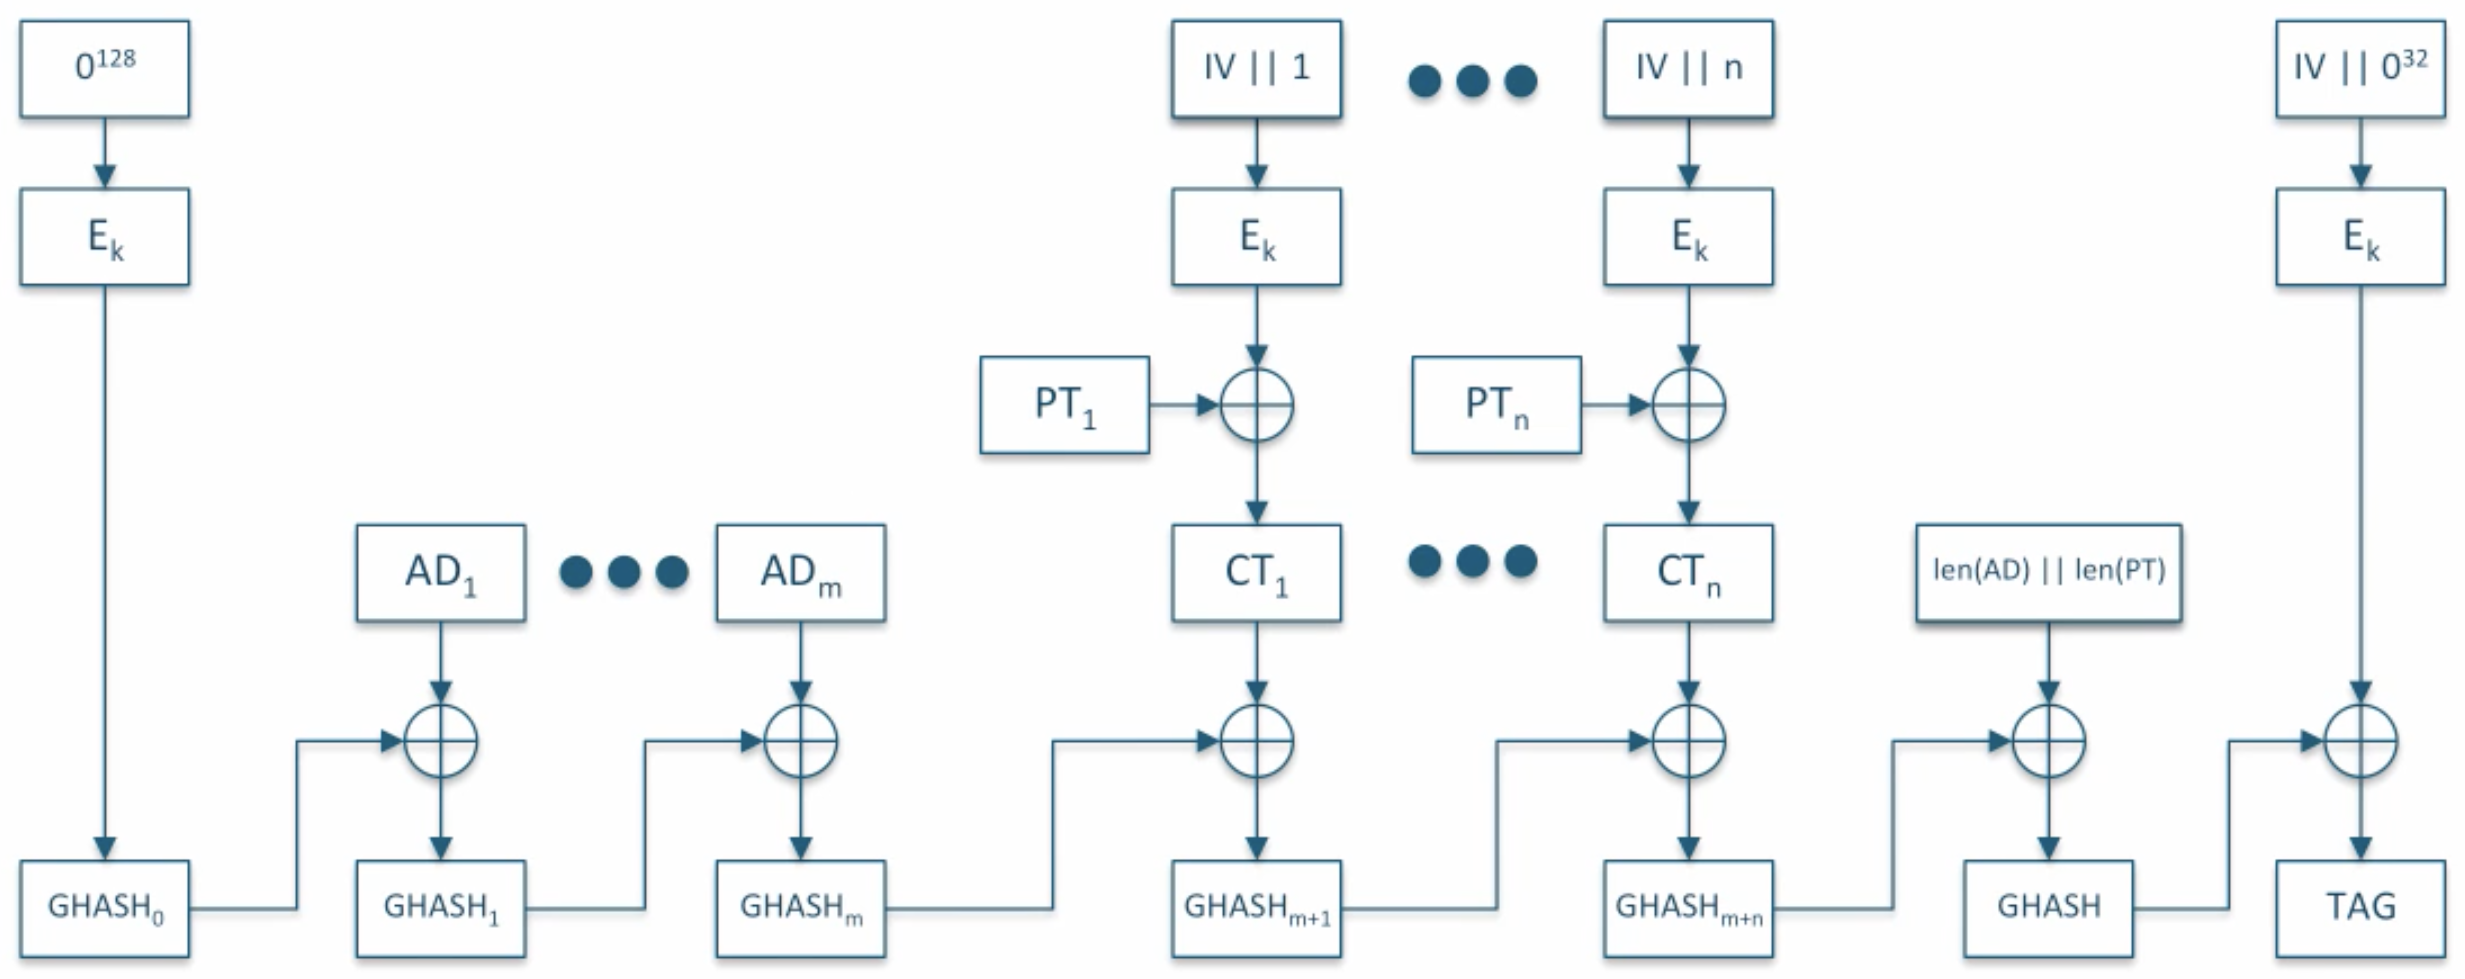
\includegraphics[width=1\textwidth]{pic1-hw3-1635747}
  \label{fig:GCM}
\end{figure}

{\em Galois Message Authentication Code (GMAC)} is an authentication-only variant of the GCM which can be used as an incremental message authentication code. Both GCM and GMAC can accept initialization vectors of arbitrary length.

\begin{figure}[!ht]
  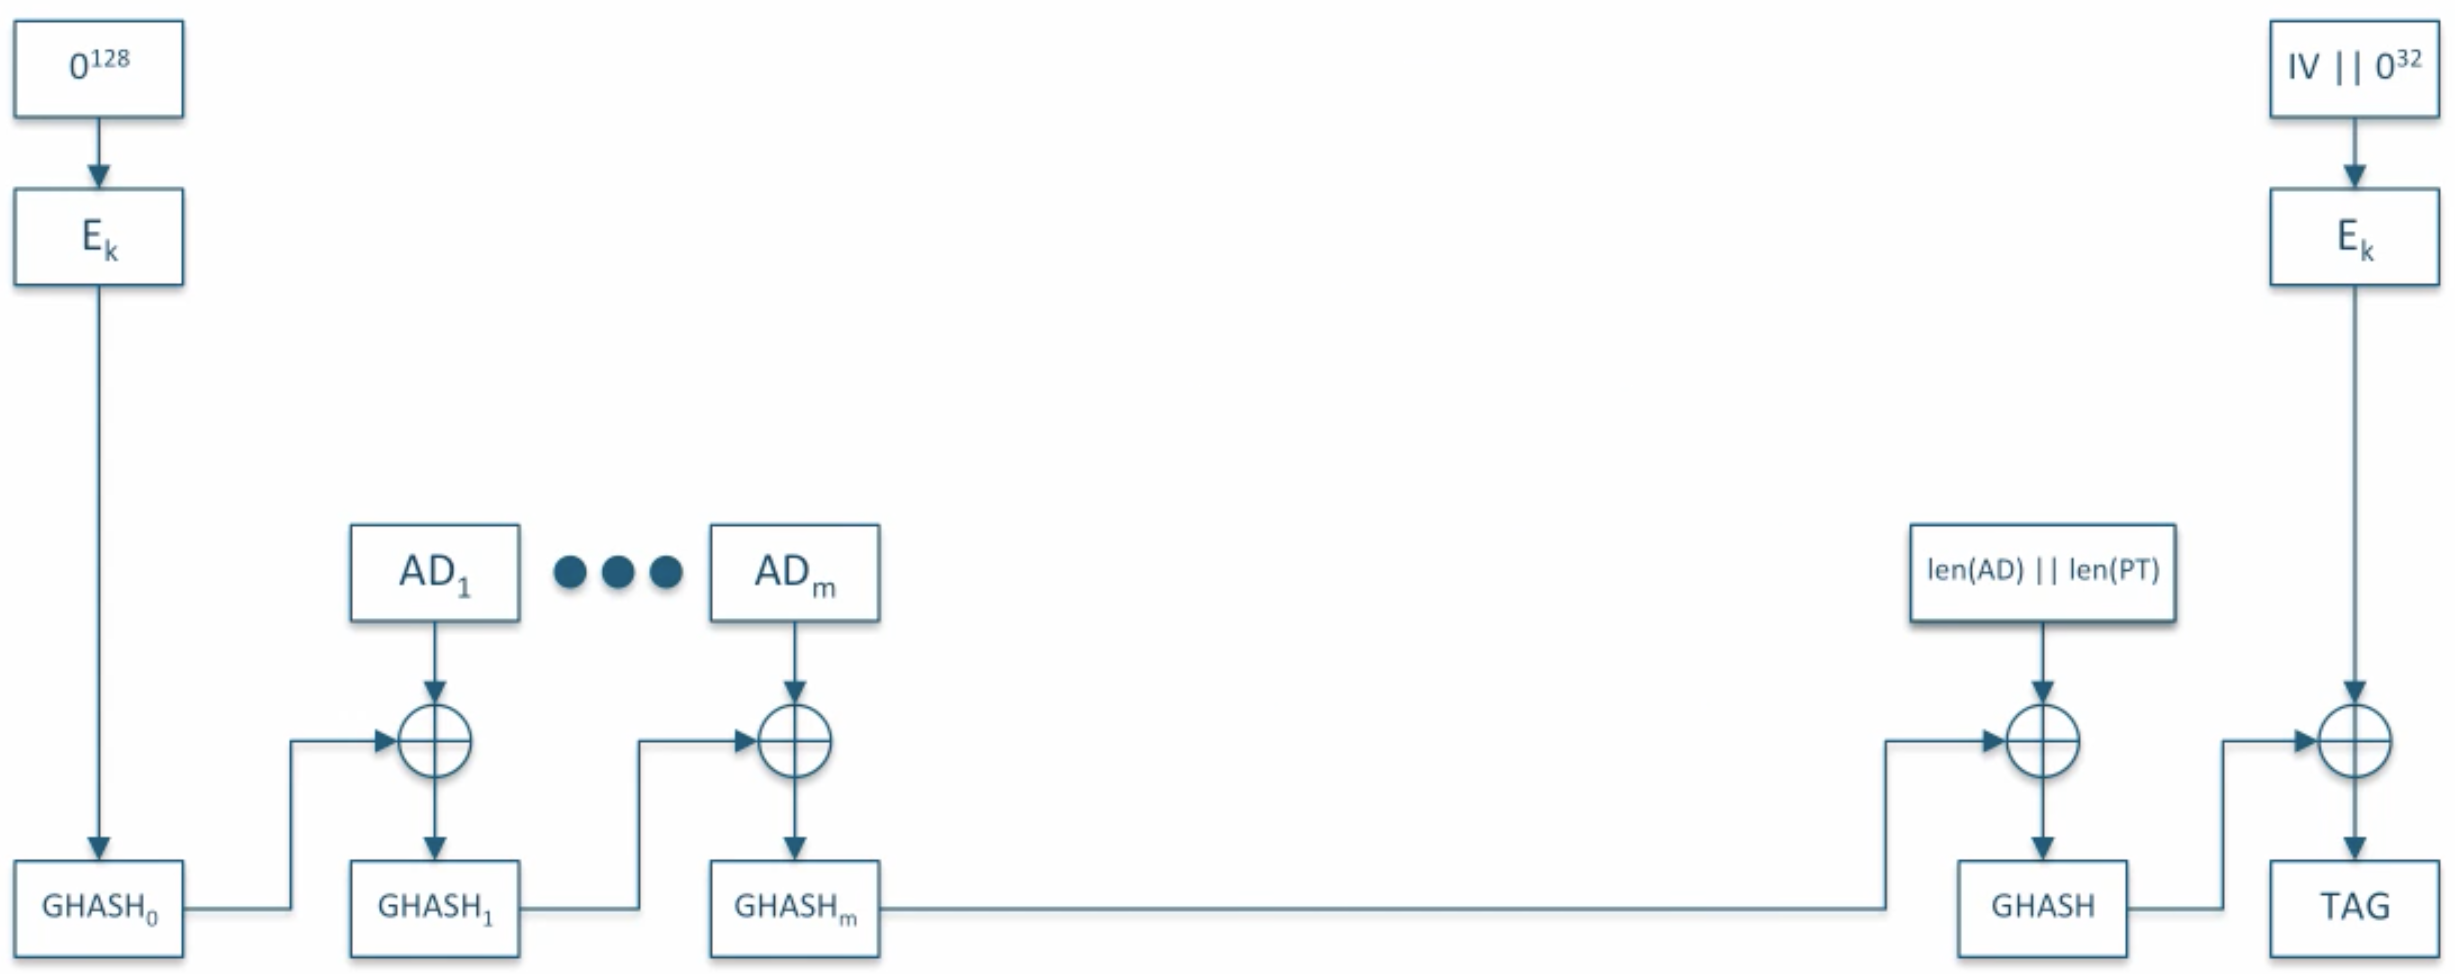
\includegraphics[width=1\textwidth]{pic2-hw3-1635747}
  \label{fig:GMAC}
\end{figure}

\newpage
\subsection{Understanding GCM and GMAC}
The two figures above are simpler then we think. Analyze it.

As we know a common method to encrypting data is to divide the plaintext into blocks and XOR it with a pseudo-random strings to return the ciphertext. For counter mode alghorithms the pseudo-random string is created by encrypting the output of a counter with an encryption algorithm, such as AES. Therefore for {\em n} blocks we have something like this:

\begin{figure}[hbt!]
  \centering
  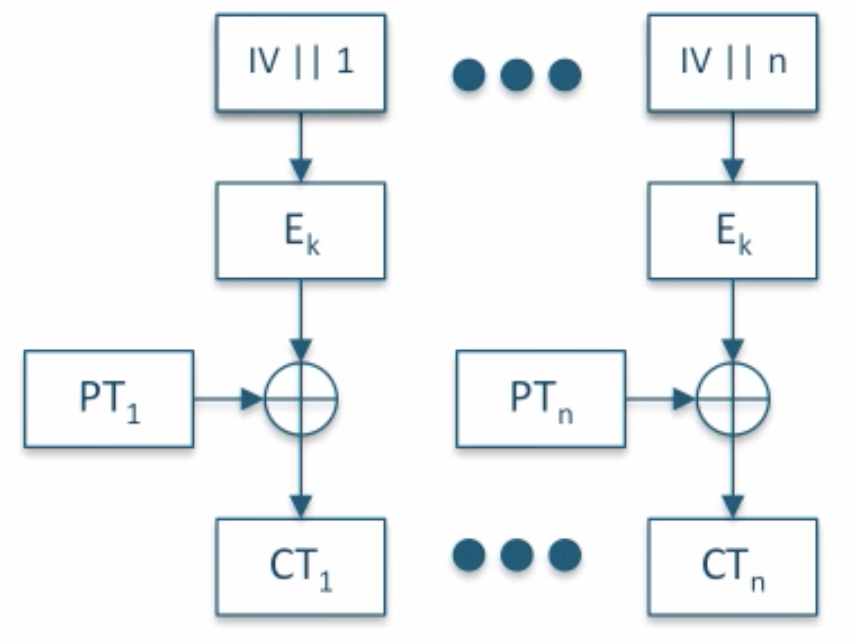
\includegraphics[width=.40\textwidth, height=.2\textheight]{pic3-hw3-1635747}
  \label{fig:Counter Mode}
\end{figure}

where the initialization vectors are used to ensure the randomness. For GCM the default length of the IV is 96 bits and the counter is 32 bits created for the 128-bits block of AES encryption.

If all we want is to encrypt the data then we have done, but we also need to ensure the integrity. For doing this we feed the ciphertext first into a XOR and then through a hashing function, after we feed the result of one stage onto the next stage of the algorithm.
\begin{figure}[hbt!]
  \centering
  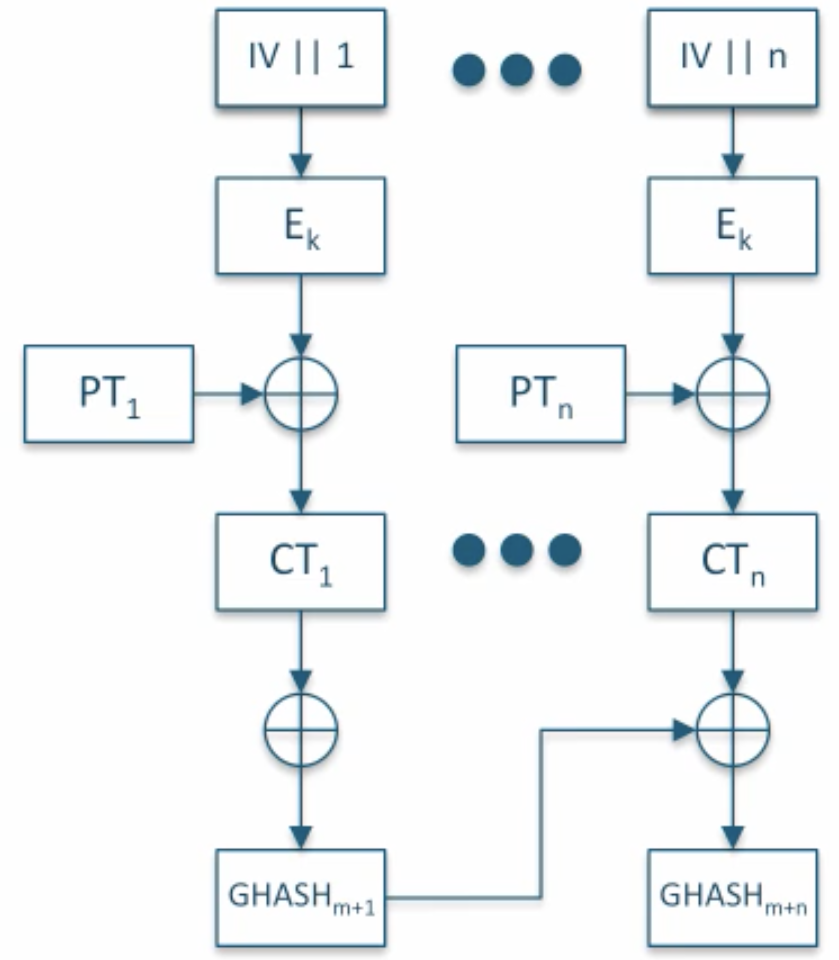
\includegraphics[width=.50\textwidth, height=.35\textheight]{pic4-hw3-1635747}
  \label{fig:Hashing function for AD}
\end{figure}
\newpage
Now we need some initial state for the hash and that is providing by sending 128 bits of 0 through the AES encryption algorithm and through the hashing function, in addition the length of plaintext (through a block) is added to the hash, finally at the end of procedures we add the initialization vector and now we have our final tag.

\begin{figure}[hbt!]
  \centering
  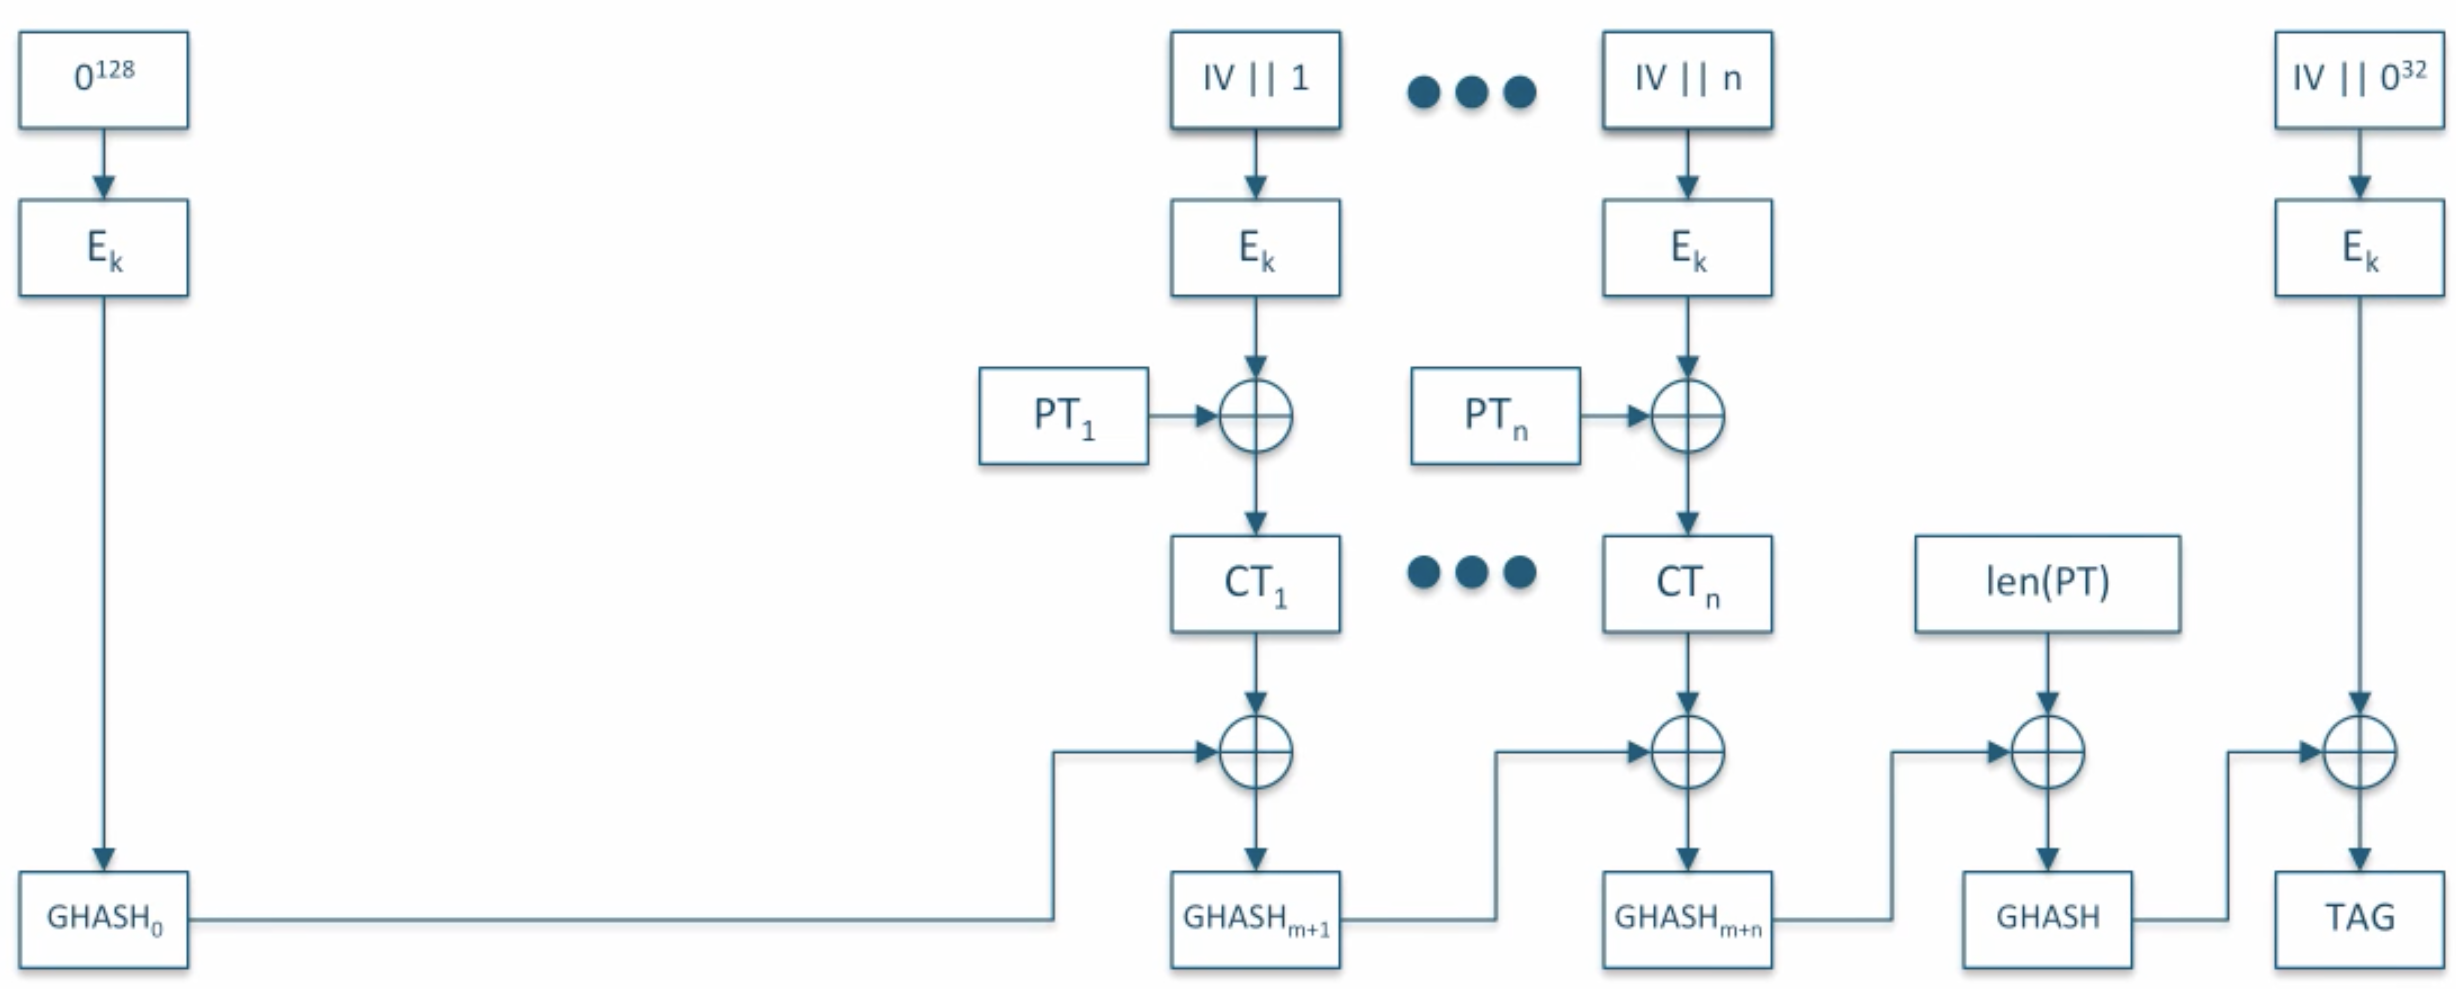
\includegraphics[width=1\textwidth]{pic5-hw3-1635747}
  \label{fig:GCM for AD}
\end{figure}

When we talk about the Galois/Counter mode this is typically what we talking about. However GCM can also be used just to authenticate the data without encrypting it. This is referred to the {\em associated data} and with these we return at the initial flowchart.

\begin{figure}[!ht]
  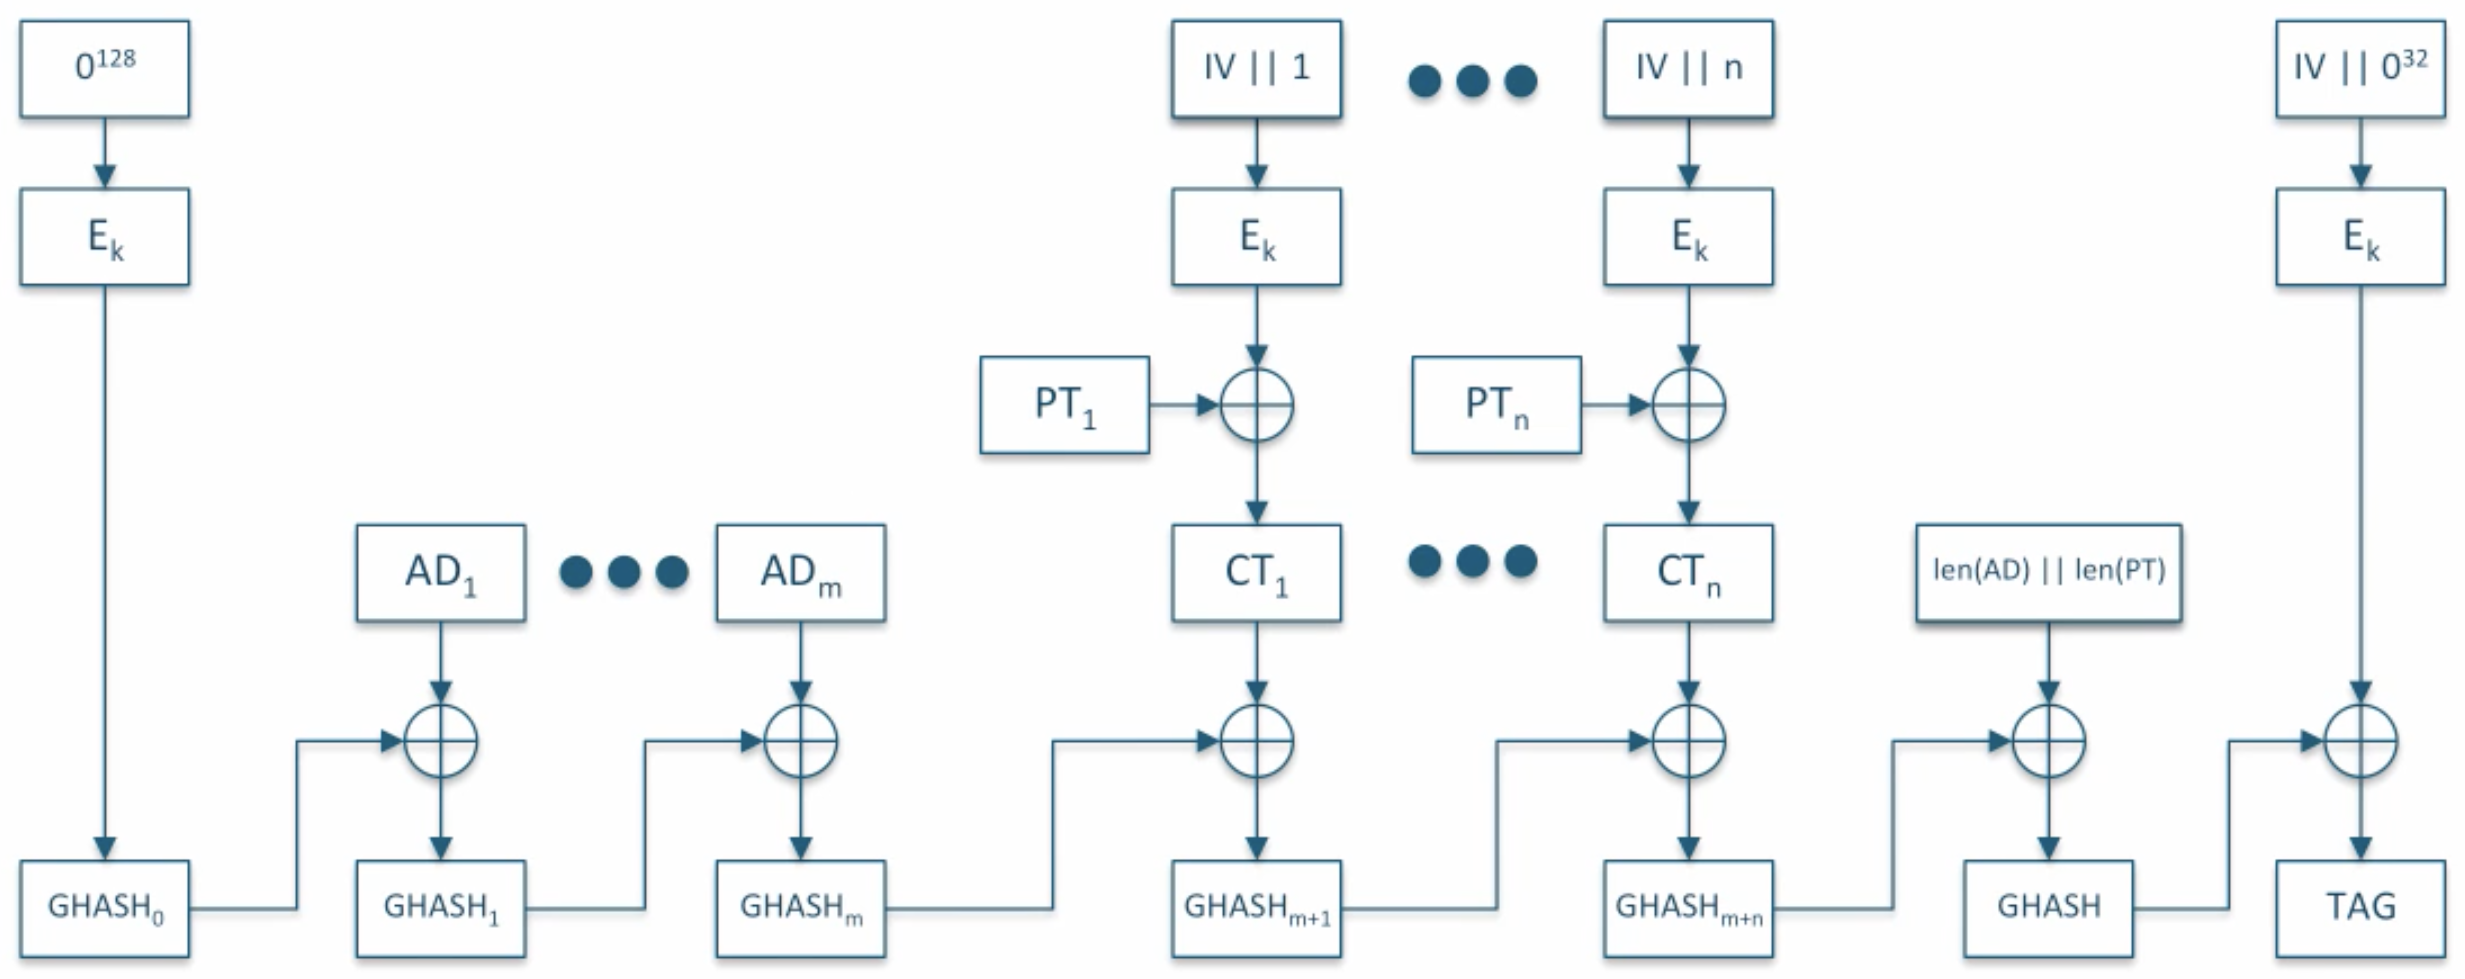
\includegraphics[width=1\textwidth]{pic1-hw3-1635747}
  \label{fig:GCM2}
\end{figure}
The authenticated {\em decryption} operation is similar to the encryption, but with the order of the hash step and encrypt step reversed. The tag that is computed by the decryption operation is compared to the tag associated with the ciphertext. If the two tags match (in both length and value), then the ciphertext is returned.

\subsection{Operating Details}
GCM combines the well-known counter mode of encryption with the new Galois mode of authentication. The key feature is that the Galois field multiplication used for authentication can be easily computed in parallel. This option permits higher throughput than authentication algorithms, like CBC, which use chaining modes. The GF($2^{128}$) field used is defined by the polynomial:

\bigskip
$ x^{128} + x^7 + x^2 + x + 1 $
\bigskip

The authentication tag is constructed by feeding blocks of data into the GHASH function and encrypting the result. This GHASH function is defined by

\bigskip
$ GHASH(H,A,C)=X_{m+n+1} $
\bigskip

where $ H = E_k(0^{128}) $ is the Hash Key, a string of 128 zero bits encrypted using the block cipher, {\em A} is data which is only authenticated (not encrypted), {\em C} is the ciphertext, {\em m} is the number of 128-bit blocks in A (rounded up), {\em n} is the number of 128-bit blocks in C (rounded up), and the variable $ X_i\;for\;i = 0, ..., m + n + 1 $ is defined as follows.

First, the authenticated text and the cipher text are separately zero-padded to multiples of 128 bits and combined into a single message $S_i$:

$$ S_i =
\Bigg \{
\begin{array}{ll}
A_i & for\;i = 1,...,m-1 \\
{A^*}_m\;||\;0^{128-v} & for\;i = m \\
C_{i-m} & for\;i = m+1,...,m+n-1 \\
{C^*}_n\;||\;0^{128-u} & for\;i = m+n \\
len(A)\;||\;len(C) & for\;i = m+n+1\\
\end{array}
$$

where {\em len(A)} and {\em len(C)} are the 64-bit representations of the bit lengths of A and C, respectively, $v\;=\;len(A)\;mod 128 $ is the bit length of the final block of A, $u\;=\;len(C)\;mod 128$ is the bit length of the final block of C, and $||$ denotes concatenation of bit strings.

Then $X_i$ is defined as:

$$ X_i = \sum_{j=1}^i S_j\cdot H^{i-j+1} =
\Bigg \{
\begin{array}{ll}
0 & for\;i = 0 \\
(X_{i-1} \oplus S_i)\cdot H & for\;i = 1,...,m+n+1 \\
\end{array}
$$

The second form is an efficient iterative algorithm (each $X_i$ depends on $X_{i-1}$). Only the final $X_{m+n+1}$ is retained as output.

If it is necessary to parallelize the hash computation, this can be done by interleaving k times:

$$ X'_i =
\Bigg \{
\begin{array}{ll}
0 & for\;i \leq 0 \\
(X'_{i-k} \oplus S_i)\cdot H^k & for\;i = 1,...,m+n+1-k \\
\end{array}
$$

$$ X_i = \sum_{j=1}^k (X'_{i+j-2k} \oplus S_{i+j-k}) \cdot H^{k-j+1} $$

{\em Note: we took this part from Wikipedia[2] without reworking it because it was already exhaustive and easy to understand}

\subsection{Parallelization more closely}
The tag computation is essentially:

\begin{itemize}
  \item Assemble A, C, $ len(A) || lenc(C) $ and Encrypt into a series of values $ x_n, x_{n-1}, x_{n-2},...,x_0 $
  \item Compute the polynomial $ x_n h^n + x_{n-1} h^{n-1} + x_{n-2} h{n-2} + ... + x_0 h^0 $
\end{itemize}

This computation is evaluated within the field GF($2^{128}$). Since it is a field, all the standard ways of rearranging the polynomial work.
For example, if we wanted to convert this into a three-way parallelism, we could compute $j=h^3$ and then the three polynomials in parallel:

$$
\begin{array}{l}
tag_2 = j^0 x_2 + j^1 x_5 + j^2 x_8 + ... \\
tag_1 = j^0 x_1 + j^1 x_4 + j^2 x_7 + ... \\
tag_0 = j^0 x_0 + j^1 x_3 + j^2 x_6 + ... \\
\end{array}
$$

and then combine them for the final result $ tag = h^2 tag_2 + h^1 tag_1 + h^0 tag_0 $.

Obviously, we can tune this to whatever degree of parallelism that suits us, and we haven't changed the tag result in any way.

\subsection{Security}
The results of GCM is the {\em Authentication Tag} and this is essential for ensure the integrity of the data. In fact if we changing a bit in the ciphertext we will have a fail in the decryption beacause the tag obteined would not correspond to the original one.

However as with any message authentication code if the adversary chooses a tag of {\em t} bits at random, it is expected to be correct for given data with probability measure $2^{-t}$. Furthermore with GCM an adversary can increase the likelihood of success by choosing only the tags with n words (the total length of the ciphertext plus any additional authenticated data (AAD)) with probability measure $2^{-t}$ by a factor of {\em n}. Although, one must bear in mind that these optimal tags are still dominated by the algorithm's survival measure $1 - n\cdot2^{-t}$ for arbitrarily large {\em t}. Moreover, GCM is neither well suited for use with very short tag lengths nor very long messages.[2]

If {\em n} denotes the total number of blocks in the encoding (the input to the GHASH function), then there is a method of constructing a targeted ciphertext forgery that is expected to succeed with a probability of approximately $ n\cdot2^{-t}$. If the tag length {\em t} is shorter than 128, then each successful forgery in this attack increases the probability that subsequent targeted forgeries will succeed, and leaks information about the hash subkey, H. Eventually, H may be compromised entirely and the authentication assurance is completely lost.[2]

Independent of this attack, an adversary may attempt to systematically guess many different tags for a given input to authenticated decryption and thereby increase the probability that one (or more) of them, eventually, will be accepted as valid. For this reason, the system or protocol that implements GCM should monitor and, if necessary, limit the number of unsuccessful verification attempts for each key.[2]

Now that we have learned how GCM works we are ready for our experiments.

\section{Experimentation}
The following is a comparison between the {\em Galois/Counter mode} (GCM) and {\em Cipher block chaining} mode (CBC). As encryption algorithm we choose {\em AES} and we measure the encryption/decryption speeds on files of different sizes: {\em 100 KB, 1 MB, 10 MB, 100 MB}. The main parameter on which we based our analysis is the {\em Average Speed Ratio}.

\bigskip
$ Average\;Speed\;Ratio = (Avg\;Speed\;Encyption)/(Avg\;Speed\;Decryption) $
\bigskip

The comparison has been conducted with the OpenSSL library using C language with a MacBook pro, Intel core i7 processor, and 8GB of RAM. The speed is measured in seconds.

First of all analyze the encypting time and the decrypting time:

\begin{figure}[hbt!]
  \centering
  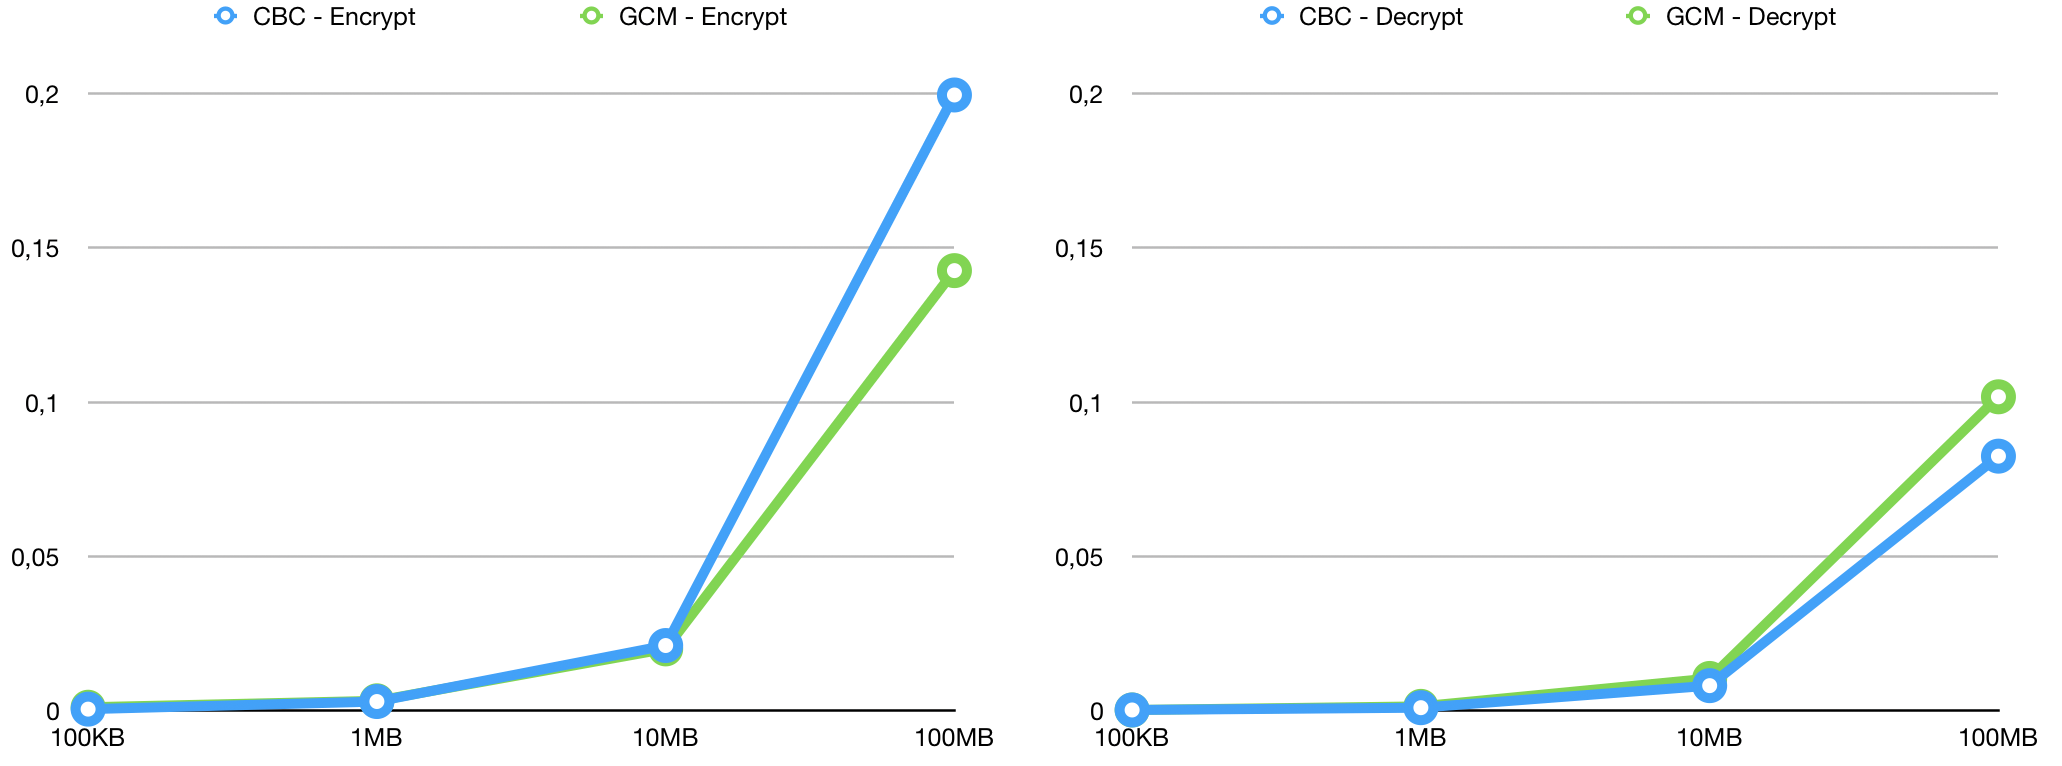
\includegraphics[width=1\textwidth]{pic6-hw3-1635747}
  \label{fig:enc-dec speed}
\end{figure}

As we can see in the figure, for the smaller files CBC and GCM behave almost equally. But with the file of 100 MB the result says us that CBC has the best speed in the decryption instead GCM has the best speed in the encryption. This means that with GCM we improve the performances of the encryption.

About the average speed ratio we have te following results:

\begin{figure}[hbt!]
  \centering
  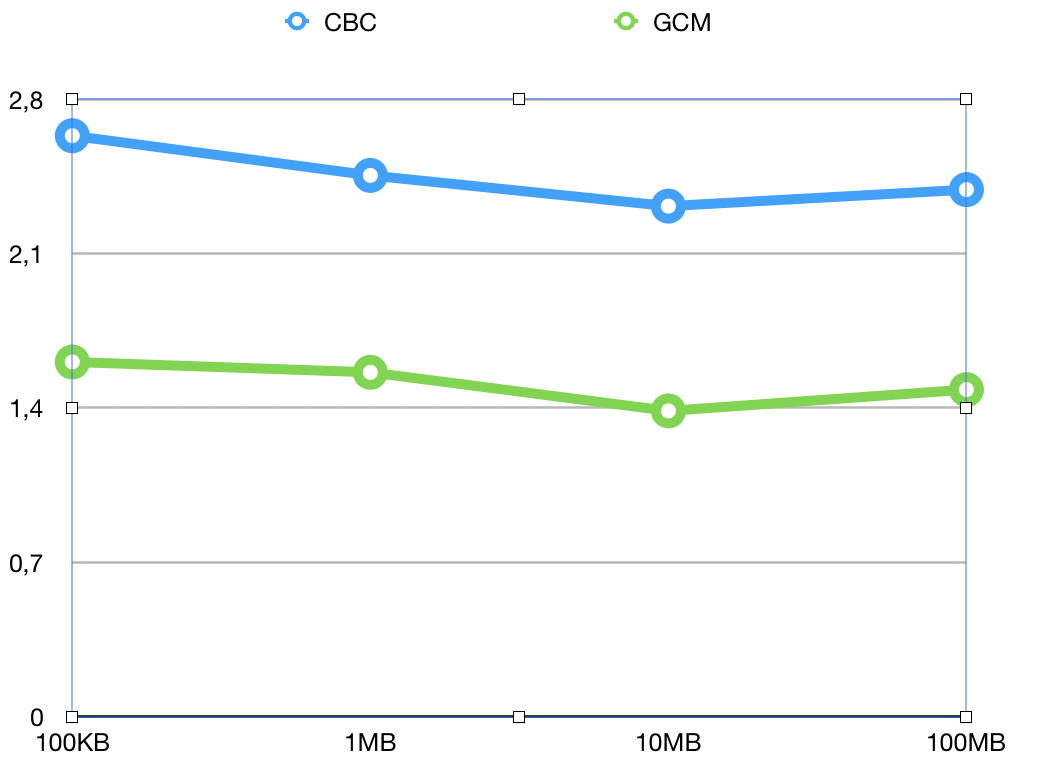
\includegraphics[width=.8\textwidth]{pic7-hw3-1635747}
  \label{fig:speed ratio}
\end{figure}

So with GCM we have slightly decreased the speed difference between the encrypt and the decrypt compared to CBC.

\section{Conclusion}
The Galois/Counter combines the well-known counter mode of encryption with the new Galois mode of authentication. It increase the performances of encryption but have a very powerfull speed also for the decryption. It is used with AES algorithm. Different block cipher modes of operation can have significantly different performance and efficiency characteristics, even when used with the same block cipher. GCM can take full advantage of parallel processing and implementing GCM can make efficient use of an instruction pipeline or a hardware pipeline. In contrast, the cipher block chaining (CBC) mode of operation incurs significant pipeline stalls that hamper its efficiency and performance. If we have to provide both integrity and confidentiality of data GCM is the right way.

\vfill
\begin{thebibliography}{99}

\bibitem{wiki1}
{\em Authenticated encryption - Wikipedia}. \newline
  \verb|https://en.wikipedia.org/wiki/Authenticated_encryption|

\bibitem{wiki2}
{\em Galois/Counter Mode - Wikipedia}. \newline
  \verb|https://en.wikipedia.org/wiki/Galois/Counter_Mode|

\bibitem{OpenSSLwiki}
{\em EVP Authenticated Encryption and Decryption}. \newline
  \verb|https://wiki.openssl.org/index.php/EVP_Authenticated_Encryption_and_Decryption|

\bibitem{link}
{\em OpenSSL Documentation}. \newline
\verb|https://www.openssl.org/docs/manmaster/man3/|

\bibitem{video}
{\em Galois/Counter Mode (GCM) and GMAC}. \newline
\verb|https://www.youtube.com/watch?v=V2TlG3JbGp0|

\end{thebibliography}

\end{document}
